\documentclass[12pt,fleqn]{article}\usepackage{../../common}
\begin{document}
Materyel Mekaniği - 11

Üç boyutta herhangi bir yönde olabilecek bir kiriş öğesinin direngenlik
matrisini bu bölümde geliştirelim [2, sf. 281]. Bunu yapabilmek için daha önce
gördüğümüz eksenel, iki boyutlu kiriş, burulma direngenlik matrislerini
birleştireceğiz.

İki boyuttaki kirişin mekaniği bükülme alttaki gibiydi [1],

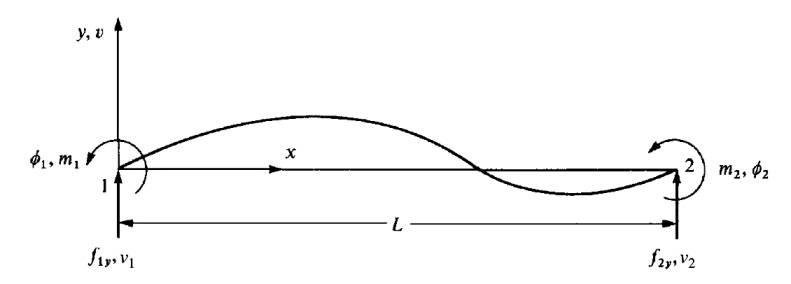
\includegraphics[width=25em]{phy_020_strs_11_02.jpg}

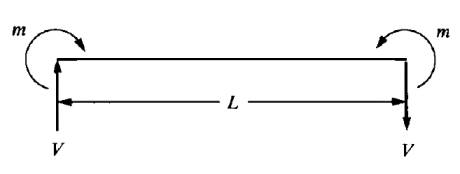
\includegraphics[width=25em]{phy_020_strs_11_03.jpg}

Şimdi işaretler alttaki gibi olacak,

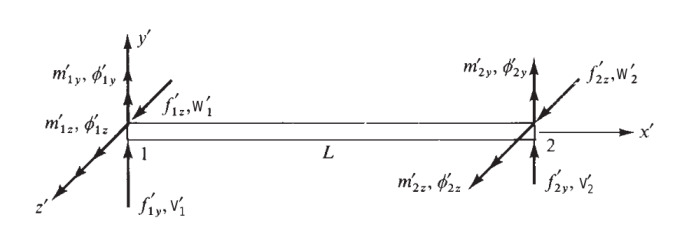
\includegraphics[width=25em]{phy_020_strs_11_01.jpg}

İki boyutlu kiriş matrisini [1] iki kez kullanacagiz, ilki $x-z$ düzlemi icin,
ikincisi $x-y$ düzlemi için,

$x-z$ düzlemi

$$
\frac{EI_y}{L^4}
\left[\begin{array}{cccc}
12L & -6L  & -12L & -6L^2 \\
    & 4L^3 & 6L^2 & 2L^3  \\
    &      & 12L  & 6L^2  \\
    &      &      & 4L^3
\end{array}\right]
\mlabel{1}
$$

$x-y$ düzlemi

$$
\frac{EI_y}{L^4}
\left[\begin{array}{cccc}
12L & 6L  & -12L & 6L^2 \\
    & 4L^3 & -6L^2 & 2L^3  \\
    &      & 12L  & -6L^2  \\
    &      &      & 4L^3
\end{array}\right]
\mlabel{2}
$$

Dikkat edersek $x-y$ düzleminin matrisi [1] matrisi ile aynı. $x-z$ düzlemi
matrisinin bazı işaretleri farklı, bunun sebebi düzlemdeki bükülmenin sağ el
kuralına göre farklı yönleri gösterebilmesi. Mesela [1]'deki 

$$
m_1 = -m = -EI \frac{\ud^2 v(0)}{\ud x^2} =
\frac{EI}{L^3} ( 6L v_1 + 4L^2 \phi_1 - 6L v_2 + 2 L^2 \phi_2 )
$$

formülünü hatırlarsak, o formülde bir uçta $m$ diğer üçta $-m$ vardı, fakat
üstteki figürde $x-z$ düzlemindeki iki uçtaki $m$ değerleri aynı işarettedir,
sağ el kuralını düşünürsek $x-z$'deki bükülme 1 noktasında kağıttan bize doğru
gösteriyor, 2 noktasında aynı şekilde. O zaman üstteki formüldeki işaretler
değişir,

$$
\Rightarrow \frac{EI}{L^3} ( -6L v_1 - 4L^2 \phi_1 + 6L v_2 - 2 L^2 \phi_2 )
$$

Bir değişim daha açılarda, üstteki formülde $\phi_1,\phi_2$ olan acılar,
üç boyuttaki üstteki şekilde bunlar $\phi_{1y}$ ve $\phi_{2y}$. Bu açılar
iki boyutlu durumun aksine artı yönde tam ters işaretli, tersi yönde bir
yer değişim $v_1,v_2$'ye sebep oluyorlarlar, bu yüzden o işaretler de
tersine dönüyor, notasyonu da düzeltince,

$$
\Rightarrow \frac{EI}{L^3} ( -6L v_1 + 4L^2 \phi_{1y} + 6L v_2 + 2 L^2 \phi_{2y} )
$$

Böylece matrisin ikinci satırında $-6,+4,+6,+2$ katsayılarını elde ediyoruz.
Bu işaretlerin (1) matrisinin ikinci satırıyla aynı olduğunu görebiliriz,
diğer satırlar benzer şekilde değiştiriliyorlar.

Üstdüşüm (Süperposition)

Artık bahsedilen matrisleri birleştirebiliriz. Bu üstdüşümü \verb!sympy!  ile
otomatik olarak yapacağız, daha önce sayısal değerler için kullandığımız
\verb!expand_dataframe! kodu yine kullanılabilecek, çünkü kod bir \verb!pandas!
Dataframe'i baz alıyor, bu Dataframe içinde herhangi bir obje depolamak mümkün,
oraya sayılar yerine \verb!sympy! sembolik matematik objeleri koyabiliriz. Bir
bonus ta elde ediyoruz, toplama işlemi \verb!sympy! tipleri için önceden
tanımlıdır, yani eğer üstdüşüm sırasında çakışma olursa, sembolik objeler
birbiriyle toplanacaktır!

\begin{minted}[fontsize=\footnotesize]{python}
from sympy import symbols, pprint, latex
from sympy.matrices import Matrix
import pandas as pd, pickle
pd.set_option('display.max_columns', None)

all_vars = ['u1','v1','w1','phi1x','phi1y','phi1z',\
            'u2','v2','w2','phi2x','phi2y','phi2z']
A,G,J,E,L,Iy,Iz = symbols("A,G,J,E,L,Iy,Iz")
\end{minted}

Önce üstte bahsedilen iki düzlemi alalım,

\begin{minted}[fontsize=\footnotesize]{python}
# x-z
vars1 = ['w1','phi1y','w2','phi2y']
M1 = pd.DataFrame([[12*L, -6*L**2,-12*L,-6*L**2],
                  [-6*L**2,4*L**3,6*L**2,2*L**3],
                  [-12*L,6*L**2,12*L,6*L**2],
                  [-6*L**2,2*L**3,6*L**2,4*L**3]],index=vars1)
M1.columns = vars1
M1 = M1 * (E*Iy/L**4 )
# x-y
vars2 = ['v1','phi1z','v2','phi2z']
M2 = pd.DataFrame([[12*L, 6*L**2,-12*L,6*L**2],
                  [6*L**2,4*L**3,-6*L**2,2*L**3],
                  [-12*L,-6*L**2,12*L,-6*L**2],
                  [6*L**2,2*L**3,-6*L**2,4*L**3]],index=vars2)
M2.columns = vars2
M2 = M2 * (E*Iz/L**4 )
\end{minted}

Şimdi [1]'deki eksenel yükleri tanımlayan makaskiriş direngenlik matrisini
alalım,

\begin{minted}[fontsize=\footnotesize]{python}
# Eksenel Yuk
vars3 = ['u1','u2']
M3 = pd.DataFrame([[1,-1],[-1,1]],index=vars3)
M3.columns = vars3
M3 = M3 * (A*E/L)
\end{minted}

[4]'te tanımladığımız burulma mekaniğinin matrisini belirtelim,

\begin{minted}[fontsize=\footnotesize]{python}
# Burulma (Torsion)
vars4 = ['phi1x','phi2x']
M4 = pd.DataFrame([[1,-1],[-1,1]],index=vars3)
M4.columns = vars4
M4 = M4 * (G*J/L)
\end{minted}

Hepsini üstdüşüm ile birleştirelim,

\begin{minted}[fontsize=\footnotesize]{python}
import sys; sys.path.append('../phy_020_strs_08')
import dfutil

M1f = dfutil.expand_dataframe(M1,all_vars)
M2f = dfutil.expand_dataframe(M2,all_vars)
M3f = dfutil.expand_dataframe(M3,all_vars)
M4f = dfutil.expand_dataframe(M4,all_vars)
Mall = M1f + M2f + M3f + M4f
pickle.dump(Matrix(Mall),open("Mall.pkl","wb"))
\end{minted}

Sonuç matrisini bir dosyaya yazalım, 

\begin{minted}[fontsize=\footnotesize]{python}
Mall = Mall.apply(np.vectorize(lambda x: latex(x)))
fout = open('matrix1.tex','w')
fout.write ('$$\n\\left[\\begin{array}{cccccccccccc}')
fout.write('\n')
for x,y in Mall.iterrows():
   row = ' & '.join(list(y)) + '\\\\'
   row = row.replace('0.0','0')
   fout.write(row)
   fout.write('\n')
fout.write ('\\end{array}\\right]\n$$')
fout.close()
\end{minted}

Ve kodu belgeye dahil edelim, matris alttaki gibi olacak,

$$
\left[\begin{array}{cccccccccccc}
\frac{A E}{L} & 0 & 0 & 0 & 0 & 0 & - \frac{A E}{L} & 0 & 0 & 0 & 0 & 0\\
0 & \frac{12 E Iz}{L^{3}} & 0 & 0 & 0 & \frac{6 E Iz}{L^{2}} & 0 & - \frac{12 E Iz}{L^{3}} & 0 & 0 & 0 & \frac{6 E Iz}{L^{2}}\\
0 & 0 & \frac{12 E Iy}{L^{3}} & 0 & - \frac{6 E Iy}{L^{2}} & 0 & 0 & 0 & - \frac{12 E Iy}{L^{3}} & 0 & - \frac{6 E Iy}{L^{2}} & 0\\
0 & 0 & 0 & \frac{G J}{L} & 0 & 0 & 0 & 0 & 0 & - \frac{G J}{L} & 0 & 0\\
0 & 0 & - \frac{6 E Iy}{L^{2}} & 0 & \frac{4 E Iy}{L} & 0 & 0 & 0 & \frac{6 E Iy}{L^{2}} & 0 & \frac{2 E Iy}{L} & 0\\
0 & \frac{6 E Iz}{L^{2}} & 0 & 0 & 0 & \frac{4 E Iz}{L} & 0 & - \frac{6 E Iz}{L^{2}} & 0 & 0 & 0 & \frac{2 E Iz}{L}\\
- \frac{A E}{L} & 0 & 0 & 0 & 0 & 0 & \frac{A E}{L} & 0 & 0 & 0 & 0 & 0\\
0 & - \frac{12 E Iz}{L^{3}} & 0 & 0 & 0 & - \frac{6 E Iz}{L^{2}} & 0 & \frac{12 E Iz}{L^{3}} & 0 & 0 & 0 & - \frac{6 E Iz}{L^{2}}\\
0 & 0 & - \frac{12 E Iy}{L^{3}} & 0 & \frac{6 E Iy}{L^{2}} & 0 & 0 & 0 & \frac{12 E Iy}{L^{3}} & 0 & \frac{6 E Iy}{L^{2}} & 0\\
0 & 0 & 0 & - \frac{G J}{L} & 0 & 0 & 0 & 0 & 0 & \frac{G J}{L} & 0 & 0\\
0 & 0 & - \frac{6 E Iy}{L^{2}} & 0 & \frac{2 E Iy}{L} & 0 & 0 & 0 & \frac{6 E Iy}{L^{2}} & 0 & \frac{4 E Iy}{L} & 0\\
0 & \frac{6 E Iz}{L^{2}} & 0 & 0 & 0 & \frac{2 E Iz}{L} & 0 & - \frac{6 E Iz}{L^{2}} & 0 & 0 & 0 & \frac{4 E Iz}{L}\\
\end{array}\right]
$$

Bu matrisin [2, sf. 282]'deki matris ile aynı olduğunu göreceğiz.

Problem 5.8

\begin{minted}[fontsize=\footnotesize]{python}
from sympy.matrices import Matrix
from sympy import symbols
import pickle

A,G,J,E,L,Iy,Iz = symbols("A,G,J,E,L,Iy,Iz")
Mall = pickle.load(open('Mall.pkl','rb'))

D = {E: 30000, G: 10000, J:50, Iy:100, Iz:100, A:10, L:100}
M = Mall.subs(D)
print (latex(M)[:100], '..')
\end{minted}

\begin{verbatim}
\left[\begin{array}{cccccccccccc}3000 & 0.0 & 0.0 & 0.0 & 0.0 & 0.0 & -3000 & 0.0 & 0.0 & 0.0 & 0.0  ..
\end{verbatim}

$$
{\scriptsize
\left[\begin{array}{cccccccccccc}3000 & 0.0 & 0.0 & 0.0 & 0.0 & 0.0 & -3000 & 0.0 & 0.0 & 0.0 & 0.0 & 0.0\\0.0 & 36 & 0.0 & 0.0 & 0.0 & 1800 & 0.0 & -36 & 0.0 & 0.0 & 0.0 & 1800\\0.0 & 0.0 & 36 & 0.0 & -1800 & 0.0 & 0.0 & 0.0 & -36 & 0.0 & -1800 & 0.0\\0.0 & 0.0 & 0.0 & 5000 & 0.0 & 0.0 & 0.0 & 0.0 & 0.0 & -5000 & 0.0 & 0.0\\0.0 & 0.0 & -1800 & 0.0 & 120000 & 0.0 & 0.0 & 0.0 & 1800 & 0.0 & 60000 & 0.0\\0.0 & 1800 & 0.0 & 0.0 & 0.0 & 120000 & 0.0 & -1800 & 0.0 & 0.0 & 0.0 & 60000\\-3000 & 0.0 & 0.0 & 0.0 & 0.0 & 0.0 & 3000 & 0.0 & 0.0 & 0.0 & 0.0 & 0.0\\0.0 & -36 & 0.0 & 0.0 & 0.0 & -1800 & 0.0 & 36 & 0.0 & 0.0 & 0.0 & -1800\\0.0 & 0.0 & -36 & 0.0 & 1800 & 0.0 & 0.0 & 0.0 & 36 & 0.0 & 1800 & 0.0\\0.0 & 0.0 & 0.0 & -5000 & 0.0 & 0.0 & 0.0 & 0.0 & 0.0 & 5000 & 0.0 & 0.0\\0.0 & 0.0 & -1800 & 0.0 & 60000 & 0.0 & 0.0 & 0.0 & 1800 & 0.0 & 120000 & 0.0\\0.0 & 1800 & 0.0 & 0.0 & 0.0 & 60000 & 0.0 & -1800 & 0.0 & 0.0 & 0.0 & 120000\end{array}\right]
}
$$


Kaynaklar

[1] Bayramlı, {\em Fizik, Materyel Mekaniği 7}

[2] Logan, {\em A First Course in the Finite Element Method, 6th Ed}

[3] Witt {\em Concepts and Apps of FEM}

[4] Bayramlı, {\em Fizik, Materyel Mekaniği 9}

\end{document}





